\ylDisplay{Optiline süsteem} % Ülesande nimi
{Tundmatu autor} % Autor
{lõppvoor} % Voor
{2017} % Aasta
{P 1} % Ülesande nr.
{2} % Raskustase
{
% Teema: Valgusõpetus
\ifStatement
Optiline süsteem koosneb kumerpeeglist ja kumerläätsest. Valguspunkt (taskulambipirni hõõgniit) asub kumerläätse optilisel peateljel läätsest kaugemal kui läätse fookuskaugus. Konstrueerige optilise süsteemi joonis, kus valguspunkti kujutis tekiks läätse fookusesse läätse ees. Selgitage lahendust.
\fi
\ifHint
Et kujutis tekiks peegli ees peegli fookuses, peavad peeglilt peegeldunud ja läätsele langevad kiired olema paralleelsed.
\fi
\ifSolution
\begin{center}
	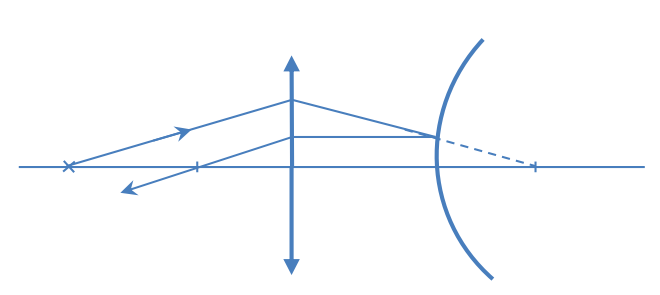
\includegraphics[width=0.5\linewidth]{2017-v3p-01-lah.PNG}
\end{center}
Et kujutis tekiks peegli ees peegli fookuses, peavad peeglilt peegeldunud ja läätsele langevad kiired olema paralleelsed. Kumerpeeglilt peegelduvad paralleelsetena kiired, mis peegelduseks koonduvatele kiirtele, mille pikendus läbiks kumerpeegli fookuse peegli taga. Kumerpeegel tuleb paigutada läätse taha nii, et ühtivad läätse kujutis ja peegli fookus. Sel juhul on kumerpeeglilt peegeldunud kiired paralleelsed. Valguspunkti asukoht läätse ees peab olema kuskil optilisel peateljel ja kaugemal kui läätse fookus, sest siis on kujutis tõeline.
\fi
}
